\documentclass{article}

\usepackage{graphicx}
\usepackage{tikz}
\usepackage{tikzsymbols}
\usetikzlibrary{calc,patterns,shapes.geometric}
\pagestyle{empty}
\usepackage[margin=0pt]{geometry}
\geometry{papersize={14in,12in}}

\def\centerarc[#1](#2)(#3:#4:#5){\draw[#1] ($(#2)+({#5*cos(#3)},{#5*sin(#3)})$) arc (#3:#4:#5);}

\begin{document}
	\begin{figure}
		\centering
		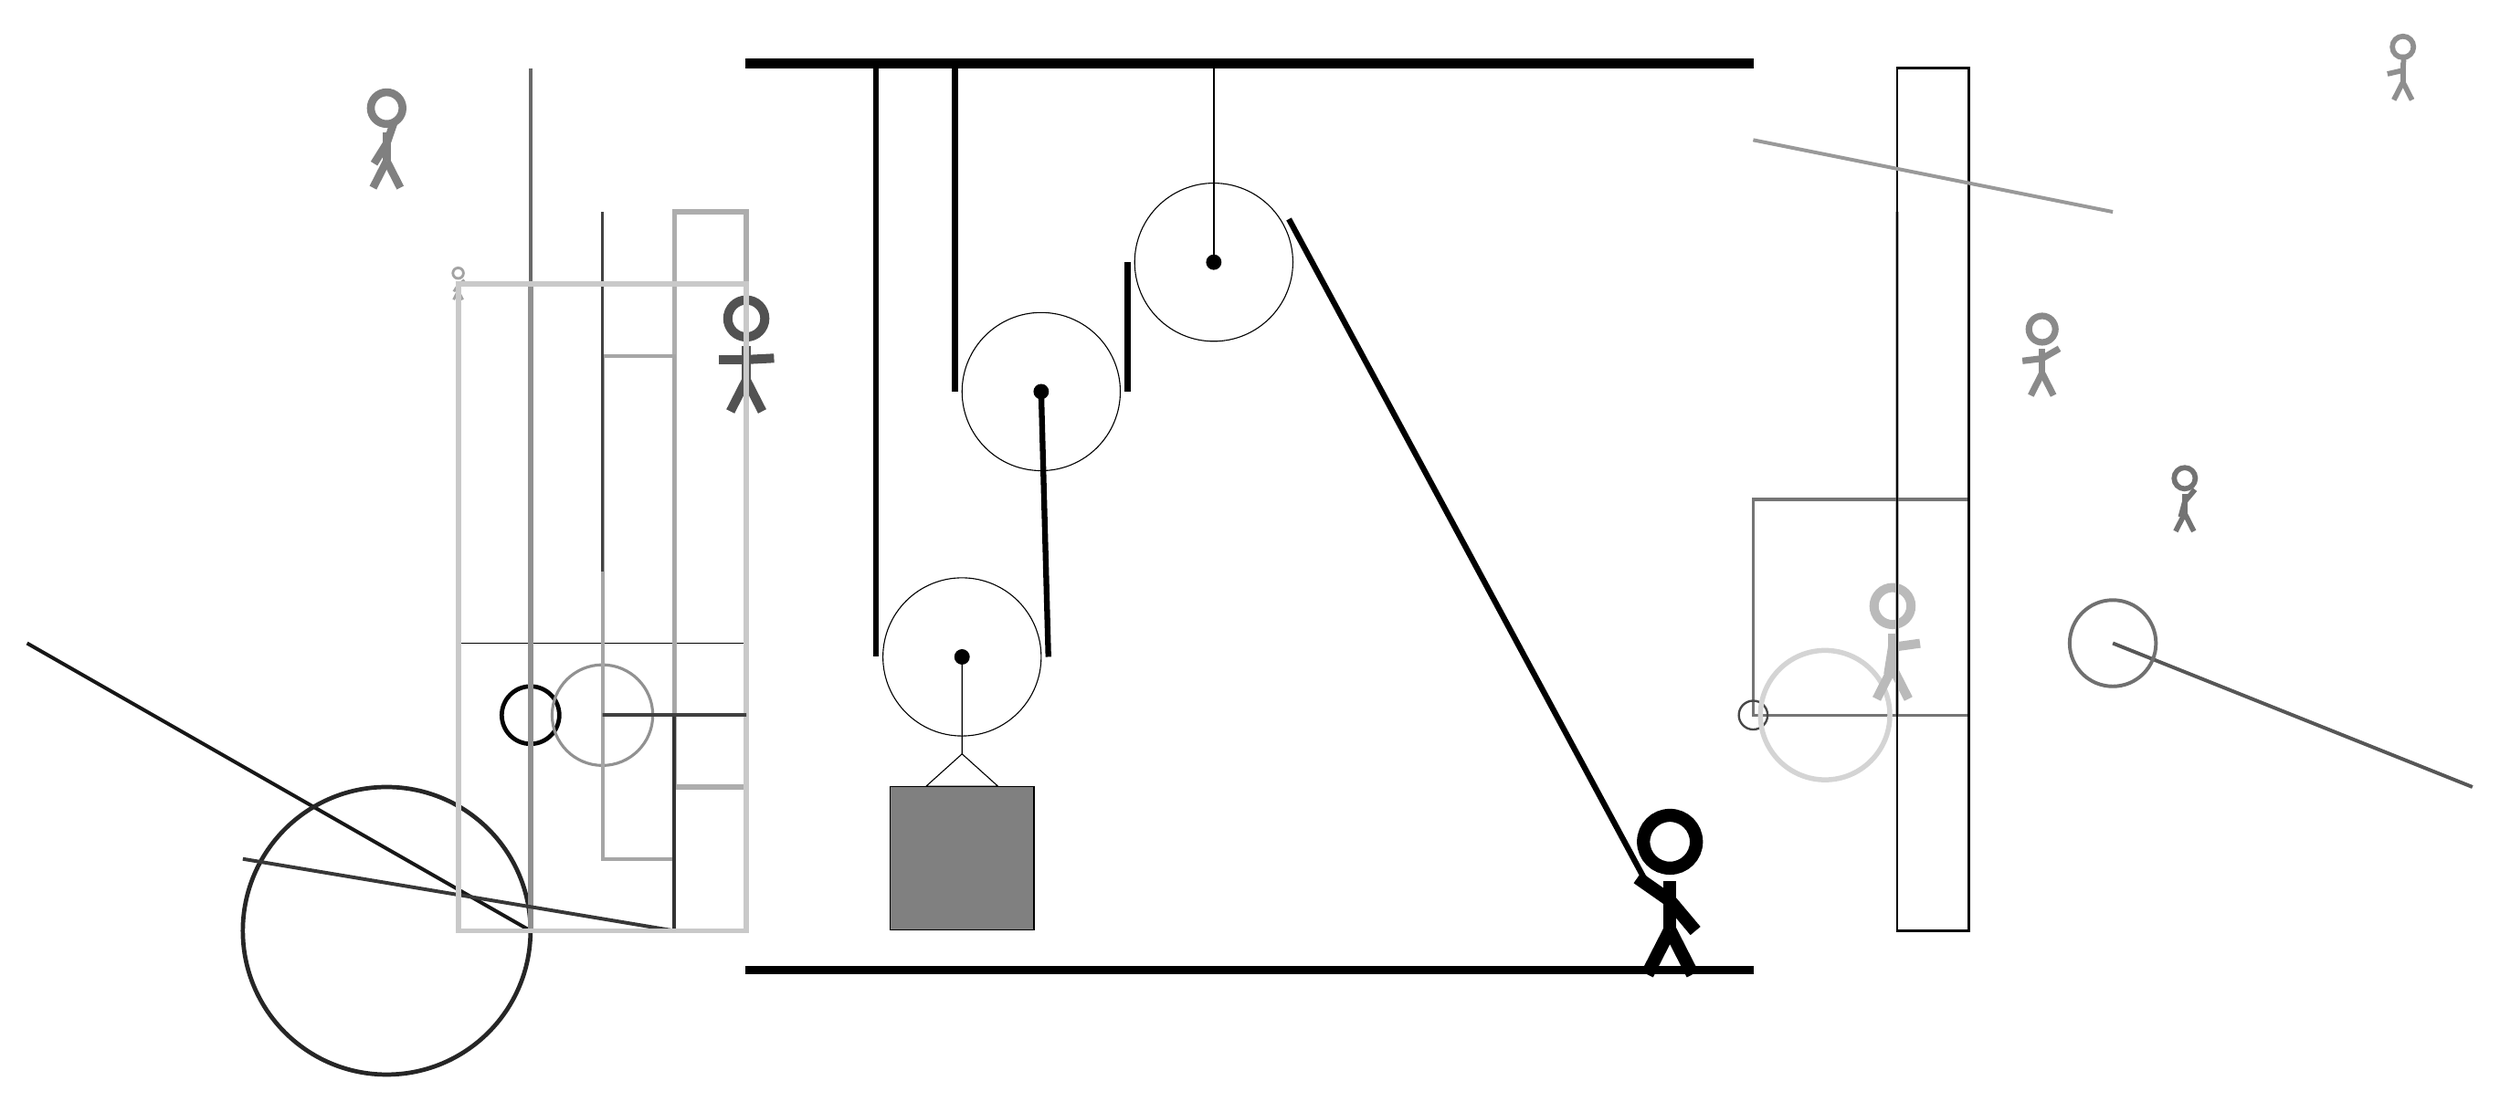
\begin{tikzpicture}
			%%%%% START %%%%%
			
			\draw[fill=black] (-2, 9) rectangle (12, 9.125);
			
			\draw (1, 0.81) circle (1.1);
			\draw[fill=black] (1, 0.81) circle (0.1);
			
			\draw (2.1, 4.5) circle (1.1);
			\draw[fill=black] (2.1, 4.5) circle (0.1);
			
			\draw[line width=0.5mm, color=black!91](-5, -3) -- (-12, 1);
			
			\draw[line width=0.5mm, color=black!29](14, 0) -- (14, 7);
			\draw[line width=0.5mm, color=black!59](-5, 9) -- (-5, -1);
			\draw[line width=0.2mm, color=black!98] (-2, -3) rectangle (-6, 1);
			
			\draw [line width=0.6mm, color=black!98](-5, 0) circle (0.4);
			
			\draw [line width=0.4mm, color=black!43](-4, 0) circle (0.7);
			\draw [line width=0.6mm, color=black!85](-7, -3) circle (2.0);
			
			\draw[line width=0.4mm, color=black!54] (12, 3) rectangle (15, 0);
			\draw [line width=0.3mm, color=black!72](12, 0) circle (0.2);
			\node[line width=0.4mm, color=black!68] at (-2, 5) {\Strichmaxerl[7][0][3]};
			\draw[line width=0.7mm, color=black!32] (-2, 7) rectangle (-3, -1);
			
			\node[line width=0.2mm, color=black!50] at (-7, 8) {\Strichmaxerl[6][58][71]};
			\draw[line width=0.7mm, color=black!43] (-2, -3) rectangle (-5, 6);
			
			\draw [line width=0.7mm, color=black!17](13, 0) circle (0.9);
			\node[line width=0.7mm, color=black!27] at (14, 1) {\Strichmaxerl[7][81][8]};
			\draw[line width=0.3mm, color=black!99] (14, 9) rectangle (15, -3);
			
			\draw[line width=0.5mm, color=black!35] (-3, -2) rectangle (-4, 5);
			\node[line width=0.5mm, color=black!36] at (-6, 6) {\Strichmaxerl[2][57][39]};
			\draw[line width=0.4mm, color=black!74] (-4, 7) rectangle (-4, 2);
			\draw[line width=0.5mm, color=black!78](-3, -3) -- (-9, -2);
			\draw[line width=0.5mm, color=black!66](17, 1) -- (22, -1);
			
			\draw[line width=0.5mm, color=black!40](17, 7) -- (12, 8);
			\node[line width=0.6mm, color=black!55] at (18, 3) {\Strichmaxerl[4][75][50]};
			\node[line width=0.3mm, color=black!46] at (16, 5) {\Strichmaxerl[5][7][30]};
			\draw [line width=0.6mm, color=black!86](15, -2) circle (0.0);
			
			\draw [line width=0.5mm, color=black!56](17, 1) circle (0.6);
			\draw[line width=0.5mm, color=black!41](15, 5) -- (15, 5);
			\draw[line width=0.5mm, color=black!80](-3, -3) -- (-3, 0);
			\draw[line width=0.7mm, color=black!21] (-2, 6) rectangle (-6, -3);
			\node[line width=0.4mm, color=black!44] at (21, 9) {\Strichmaxerl[4][13][86]};
			\draw[line width=0.5mm, color=black!75] (-2, 0) rectangle (-4, 0);
			
			
			\draw (4.5, 6.3) circle (1.1);
			\draw[fill=black] (4.5, 6.3) circle (0.1);
			\draw[thick] (4.5, 6.3) -- (4.5, 9);
			
			\draw (1, 0.81) -- (1, -0.54) -- (0.5, -0.99) -- (1.5, -0.99) -- (1, -0.54);
			\draw[fill=black!50] (0, -0.99) rectangle (2, -2.99);
			
			\draw[line width=0.8mm] (-0.2, 9) -- (-0.2, 0.81);
			\centerarc[line width=0.8mm](1, 0.81)(180:360:1.2000000000000002);
			\draw[line width=0.8mm](2.2, 0.81) -- (2.1, 4.5);
			\draw[line width=0.8mm] (0.9, 9) -- (0.9, 4.5);
			\centerarc[line width=0.8mm](2.1, 4.5)(180:360:1.2000000000000002);
			\draw[line width=0.8mm](3.3, 4.5) -- (3.3, 6.3);
			\centerarc[line width=0.8mm](4.5, 6.3)(30:180:1.2000000000000002);
			\draw[line width=0.8mm] (5.544, 6.9) -- (10.5, -2.3);
			
			\node at (10.8, -2.5) {\Strichmaxerl[10][-35][-50]};
			
			\draw[fill=black] (-2, -3.5) rectangle (12, -3.6);
			
			%%%%% END %%%%%
		\end{tikzpicture}
	\end{figure}	
\end{document}